\documentclass[mastinf,utf8,bibnum,hyperref,zihtitle,german]{zihpub}
\usepackage[ruled,vlined,german,algochapter]{algorithm2e}
\usepackage{float}
\author{Jan Philipp Simon Langen}
\title{Anwendung neoronaler Netze zur inhaltsbasierten Bildsuche bei historischen Bilddarstellungen}
\birthday{26. Dezember 1994}
\placeofbirth{Münsterlingen}
\betreuer{Dr. Christoph Lehmann \& Dr. Taras Lazariv}
\bibfiles{literatur}
\newcommand{\comment}[1]{}
\begin{document}
\setlength{\emergencystretch}{1pt}
\section*{Motivation}
Präzise und effiziente Suchwerkzeuge sind essenziell um große Datenmengen für einen Nutzer sinnvoll verwertbar zu machen. Dies gilt insbesondere auch im Bereich der Bildersuche. Die klassische Bildersuche basiert auf vom Nutzer formulierten Anfragen, mit deren Hilfe das Suchsystem eine Liste an passenden Bildkandidaten zusammenstellt und zurückgibt. Hierbei nutzt das System eine Reihe von Zusatzinformationen, sogenannten Metadaten, wie Tags, Titel, Aufnahmeort oder Datum. Eine alternativer Ansatz der Suche, der in dieser Arbeit behandelt wird, ist die inhaltsbasierte Bildersuche (engl. Content-Based Image Retrieval, kurz CBIR). Hierbei werden vom Nutzer keine Anfragen formuliert. Stattdessen dient ein Bild als Suchanfrage. Ziel ist es, Bilder mit gleichem oder ähnlichem Bildinhalt als Ergebnis zurückzugeben. Ein Vorteil dieser Herangehensweise ist, dass der Nutzer keine Informationen über den Inhalt des Suchbildes benötigt. Das System arbeitet ausschließlich mit den Pixelinformationen der Bilder. Ein weiterer Vorteil ist daher, dass weder im Suchbild noch in der Suchdatenbank Metadaten zu den Bildern vorhanden sein müssen, was die Einsatzmöglichkeiten von inhaltsbasierter Suche sehr flexibel gestaltet. Im Folgenden wird die inhaltsbasierte Suche auch als Image Retrieval bezeichnet.
\\\\
Das Anwendungsgebiet dieser Arbeit ist die Suche auf historischen Bildern. Diese weit gefasste Domäne ist besonders herausfordernd, da sie sehr heterogene Daten enthält. Dabei gibt es nicht nur große Unterschiede in den abgebildeten Bildinhalten, wie Gebäude, Naturaufnahmen oder Portraits, sondern auch in den verwendeten Aufnahmeverfahren. Durch die Fortschritte der Aufnahmetechnik können historische Bilder sowohl in Form von Zeichnungen oder Malerei, aber auch als Druck oder in anfänglichen Formen der Photographie vorliegen. Da Metadaten zu historischen Bildern erst bei der Digitalisierung hinzugefügt werden können, sind diese oft gar nicht oder nur lückenhaft vorhanden. Dies macht die inhaltsbasierte Suche für diese Domäne im Vergleich zur klassischen Bildersuche zu einer besonders geeigneten Methode. Mit der Umsetzung einer unterstützenden Suche für das UrbanHistory4D Projekt \cite{urbanhistory4d} ergibt sich ein konkreter Anwendungsfall für diese Arbeit. Das UrbanHistory4D Projekt befasst sich mit der Erstellung interaktiver Stadtkarten. Wo vorhanden kann sich der Nutzer historische Aufnahmen anzeigen lassen, die den Ort zeigen, an dem er sich innerhalb der Karte befindet. Das Akkumulieren und Zuordnen von historischen Bildern zu diesen Plätzen ist ein wesentlicher Arbeitsanteil bei der Erstellung der Karten. Image Retrieval Systeme können helfen den Suchaufwand für die Ersteller der Karten signifikant zu reduzieren. Dabei handelt es sich um einen aktiven Forschungsbereich, in dem momentan unterschiedliche Suchsysteme analysiert werden. 
\\\\
Das Image Retrieval Verfahren DELF (attentive DEep Local Features) \cite{delf} entwickelt von Noh, \mbox{Araujo} et al., welches in dieser Arbeit untersucht wird ist ein Deep Learning Ansatz. Durch den raschen Fortschritt im Bereich tiefer neuronaler Netzwerkarchitekturen der letzten Jahre erfreuen sich gelernte Ansätze immer größerer Beliebtheit. DELF erzielt auf bekannten Benchmarkdatensätzen wie Oxford5k \cite{oxford5k} und Paris6k \cite{paris6k} sehr gute Ergebnisse. Besonders gut schneidet DELF im Vergleich auf dem eigens erstellten Google Landmarks Datensatz \cite{landmarks} ab. Dieser enthält mit über 1 Mio. Bilder und 13k unterschiedlichen Motiven eine deutlich heterogenere Mischung an Objekten als andere Benchmarks. Die gute Performanz auf diesem Datensatz lässt also hoffen, dass sich das DELF-Verfahren auch für die historische Domäne eignet.



%\newpage
\chapter{Verwandte Arbeiten}\label{related_work}
Bei Information Retrieval handelt es sich um ein Problem aus dem Bereich der Computer Vision, welches bereits seit langem intensiv erforscht wird. In frühen Ansätzen versuchte man vor allem globale Beschreibungen von Bildern zu erstellen, um diese untereinander vergleichen zu können. Diese basierten zum Beispiel auf Farbhistogrammen oder Texturbeschreibungen \cite{early_days}. Allerdings waren diese Ansätze oft sehr anfällig für Unterschiede in Beleuchtung, Skalierung und anderen Transformationen, wie sie bei unterschiedlichen Aufnahmen des selben Motivs auftreten können.
\\
Ein wesentlicher Durchbruch gelang David G. Lowe 2004 mit der Entwicklung des SIFT-Verfahrens (Scale Invariant Feature Transform) \cite{sift}. Hierbei werden mehrere Konzepte vereint um Bildbeschreibungen zu erzeugen, die robuster gegenüber unterschiedlichen Transformationen sind. So arbeitet der SIFT Algorithmus beispielsweise nicht direkt auf den Bildern, sondern im sogenannten Scale Space. Dieser besteht auf unterschiedlich skalierten Versionen des Ursprungsbildes, auf welche wiederum unterschiedlich starke Gauß-Filter angewendete werden. Betrachtet werden schließlich Differenzbilder zwischen benachbarten Stärken der Gauß-Fitler Ergebnisse. Die Verwendung von unterschiedlich skalierten Bildversionen macht die berechneten SIFT-Merkmale deutlich robuster gegen Skalierungsunterschiede. Das SIFT-Verfahren besteht aus zwei Phasen. In der ersten Phase werden über die Suche nach lokalen Extrema bedeutsame Bildpunkte ausgewählt. Für diese werden in der zweiten Phase einzelne Deskriptoren berechnet. Das Bild wird also nicht global beschrieben, sondern über viele lokale Deskriptoren dargestellt. Die lokalen Deskriptoren ergeben sich aus Histogrammen der Gradientrichtungen umliegender Bildpunkte. Diese werden relativ zu der dominanten Gradientrichtung in der Umgebung berechnet, was die Deskriptoren invariant gegenüber Rotationen macht. Lowes Entwicklung bildet den Ursprung für viele abgeleitete Verfahren wie SURF\cite{surf}, PCA-SIFT\cite{pca_sift} und RIFT\cite{rift}. Auch in aktueller Forschung werden Image Retrieval Verfahren untersucht, die mit SIFT-Merkmalen arbeiten \cite{modern_sift_useage}. \\
Der Trend bei der Entwicklung neuer Image Retrieval Systeme geht aktuell jedoch hauptsächlich in Richtung von gelernten Verfahren. Die Basis dieser Verfahren bilden tiefe CNN-Architekturen (Convolutional Neural Networks). Ein neuronales Netzwerk lässt sich als eine schichtweise Aneinanderreihung nicht-linearer Funktionen auffassen. Convolutional Neural Networks sind ein Sonderfall neuronaler Netze, welche sogenannte Convolutional Layer, zu deutsch faltende Schichten, enthalten. In diesen Schichten werden Faltungs/ bzw. Filteroperationen auf die Eingabedaten angewendet, um für das Netzwerk hilfreiche Merkmale in den Daten hervorzuheben. Dies ist durchaus vergleichbar mit den Filteroperationen, die im SIFT-Verfahren verwendet werden. Der Unterschied besteht jedoch darin, dass die Parameter der verwendeten Filtermasken sowie aller anderen Netzparameter nicht per Hand gewählt, sondern in einem Trainingsverfahren für den aktuellen Anwendungsfall optimiert werden. Der Entwickler bestimmt lediglich die grobe Architektur des Netzwerks, also die Anzahl, Größe und Reihenfolge der verwendeten Schichten sowie die Art der Operationen, die in ihnen durchgeführt werden. In Image Retrieval Systemen werden CNNs eingesetzt, um Bilddeskriptoren zu erstellen. Hierfür werden Zwischenergebnisse des Netzwerks, also die Ausgaben einer bestimmten Schicht genutzt. An welcher Stelle im Netzwerk die Deskriptoren entnommen werden ist dabei von entscheidender Bedeutung. Zeiler und Fergus haben in ihrer Studie zur Visualisierung von CNNs gezeigt \cite{extraction_point_meaning}, dass die früheren Schichten von CNNs typischerweise einfache Konzepte wie Kanten oder Ecken hervorheben. Mit wachsender Tiefe der betrachteten Netzwerkschicht steigt auch die Komplexität der Konzepte, die von den Ausgaben der Schicht beschrieben werden können.
\\\\
In dem in \cite{fc_extraction_neural_codes} beschriebenen Image Retrieval System von Babenko, Slesarev et al. wird als Modell ein CNN bestehend aus fünf faltenden gefolgt von drei vollvernetzten Schichten (im Englischen fully-connected layer) genutzt. Als Deskriptoren werden die Ausgaben der ersten bzw. zweiten vollvernetzten Schicht verwendet. In einer vollvernetzten Schicht hat jeder Wert der Eingabe Einfluss auf jeden Wert in der Ausgabe. Die Ausgaben solcher Schichten werden also von der gesamten Bildeingabe beeinflusst und können daher als globale Deskriptoren verstanden werden. Diese intuitive Herangehensweise erzielt leichte Verbesserung gegenüber den zur Zeit der Veröffentlichung gängigen algorithmischen Verfahren.
\\
Razavian, Sullivan et al. stellen in \cite{convnet} ein System auf Basis der in \cite{convnetarc} beschriebenen Netzwerkarchitektur vor. Das Modell besteht ebenfalls aus fünf faltenden und drei vollvernetzten Schichten. Die Deskriptoren stammen aus den Ausgaben der letzten faltenden Schicht.
%Die Dimensionalität der Deskriptoren wird durch Anwendung einer max-pooling Operation auf 2048 Dimensionen beschränkt.
Anders als bei Babenko, Slesarev et al. werden in diesem System mehrere Deskriptoren pro Bild erstellt. Hierfür werden systematisch Teilbilder aus Bildbereichen unterschiedlicher Größe generiert. Anschließend werden die Teilbilder auf eine feste Größe skaliert und als Eingabe in das Netzwerk gegeben. So wird für jeden betrachteten Bildbereich ein eigener lokaler Deskriptor erstellt. In ihren Experimenten stellen die Autoren fest, dass die Verwendung von lokalen Deskriptoren gegenüber einer globalen Betrachtung zu einer signifikanten Verbesserung der Retrievalperformanz führt. Der überwiegende Teil aktueller Retrieval Systeme setzt auf die Erstellung von lokalen Deskriptoren.
\\
Eine interessante Frage bei der Konzeption von Image Retrieval Systemen, die mit lokalen Deskriptoren arbeiten ist, wie man entscheidet, welche Bildregionen am sinnvollsten zu betrachten sind. Das ONE-Verfahren \cite{one} von Xie, Hong et al. nutzt ein VGG-19 \cite{vgg} Modell und extrahiert Deskriptoren aus der vorletzten vollvernetzten Schicht. Als Eingaben in das Netzwerk dienen sogenannte Object Proposals. Dabei handelt es sich um Bildausschnitte, welche Regionen umschließen, in denen Objekte vermutet werden. Die Autoren testen sowohl manuell annotierte sowie automatisch extrahierte Object Proposals und erzielen mit beiden Ansätzen ähnlich gute Ergebnisse. Für die automatische Bestimmung von Object Proposals nutzen sie das Selective Search Verfahren \cite{selective_search}.
\\
Das Delf-Verfahren \cite{delf}, welches in dieser Arbeit untersucht wird, basiert ebenfalls auf lokalen Deskriptoren. Die Deskriptoren werden aus einer faltenden Schicht aus dem hinteren Teil eines ResNet-50 \cite{resnet} Modells extrahiert. Als Eingabe in das Netzwerk werden Bilder in ihrer Gesamtheit betrachtet. Da bis zur Extraktionsschicht keine vollvernetzten Schichten genutzt werden, kann für jeden extrahierten Wert zurückgerechnet werden, von welchen Bereichen des Ursprungsbildes er beeinflusst wurde. Dies erlaubt es die Ausgaben der Extraktionsschicht in einzelne lokale Deskriptoren zu unterteilen. Um auszuwählen welche der lokalen Deskriptoren zur Darstellung eines Bildes genutzt werden sollen, werden die lokalen Deskriptoren in ein weiteres neuronales Netz gegeben. Dieses Netz hat die Aufgabe zu bewerten, wie geeignet die einzelnen Deskriptoren zur Beschreibung des Gesamtbildes sind. Auf Grund dieser Bewertung werden die wichtigsten Deskriptoren zu jedem Bild ausgewählt, wogegen schlecht bewertete Deskriptoren verworfen werden. Der konzeptionelle Unterschied bei der Auswahl der Deskriptoren im Vergleich zum ONE-Verfahren ist, dass die Auswahl auf Grund der bereits berechneten Deskriptoren geschieht anstatt auf Grund des Ursprungsbildes. Die Funktionsweise des Delf-Verfahrens wird in Kapitel \ref{delf_chapter} ab Seite \pageref{delf_chapter} im Detail erklärt.
\\  
Bevor Neuronale Netze für die Erstellung von Deskriptoren genutzt werden können, müssen ihre Parameter in einem Trainingsverfahren optimiert werden. Während dem Training muss das Netzwerk eine Aufgabe lösen. Wie erfolgreich das Netzwerk dabei ist, wird mit Hilfe einer Fehlerfunktion dargestellt. Das Netz versucht seine Parameter so anzupassen, dass die Fehlerfunktion minimiert wird. Im Fall der bereits vorgestellten Verfahren wird dabei eine Dummy-Aufgabe, typischerweise die Klassifikation von Bildern, gelöst. In der letzten Zeit wurden jedoch einige Ansätze veröffentlicht, die versuchen neuronale Netze direkt an Image Retrieval Aufgaben zu trainieren. Radenović, Tolias und Chum stellen in \cite{siamac_contrastive_loss} eine solchen Ansatz vor. Während dem Training arbeiten sie dabei mit Bildpaaren $(i,j)$. Diese Paare werden als korrektes Match bezeichnet, falls sich ihre Bildinhalte überschneiden. Andernfalls handelt es sich um ein inkorrektes Match. Beide Bilder durchlaufen ein identisches Netz und erzeugen dabei jeweils eine Ausgabe $(\mathbf{d}(i),\mathbf{d}(j))$. Für die Optimierung wird eine spezielle Fehlerfunktion $L$ definiert. Falls es sich bei den Bildern um ein korrektes Match handelt, sollten sich die Netzwerkausgaben der Bilder möglichst ähneln.
\begin{equation}
L_{korr}(i,j) = \dfrac{1}{2} \parallel \mathbf{d}(i) - \mathbf{d}(j)\parallel^{2} 
\end{equation}
Handelt es sich jedoch um ein inkorrektes Match, sollten die Ausgaben einen Mindestabstand $\tau$ zueinander einhalten.
\begin{equation}
L_{inkorr}(i,j) = \dfrac{1}{2} \max\left[0, \tau - \parallel \mathbf{d}(i) - \mathbf{d}(j)\parallel^{2}\right] 
\end{equation}
Die Autoren testen ihr Verfahren auf unterschiedlichen CNN Architekturen wie VGG \cite{vgg} und AlexNet \cite{alexnet} und erzielen damit sehr gute Ergebnisse auf gängigen Retrievalbenchmarks. Das direkte Training auf Retrievalaufgaben ist eine vielversprechende neue Forschungsrichtung im Retrievalbereich, an der momentan intensiv gearbeitet wird.
\\\\
% delf gesamtes bild als input durch conv layer wird auf lokale punkte zurückgerechnet. attention training auf den deskriptoren um gute auszuwählen. näheres  im konkreten kapitel
% diese system benötigen alle einen dummy task um die netzwerke zu trainieren oder benutzen vortrainierte netze alles mit klassifikation trainiert. es gibt aber ansätze die versuchen ein direkt für einen retrieval taks zu trainieren sia mac
Da Image Retrieval Systeme meist auf großen Bilddatenbanken eingesetzt werden und somit für eine Suchanfrage viele Bilder miteinander verglichen werden müssen, ist es sinnvoll Bildrepräsentationen so kompakt wie möglich zu gestalten, um die Laufzeit der Suche zu verbessern. Insbesondere bei Verfahren, die lokale Deskriptoren erstellen und häufig hunderte oder tausende Merkmale pro Bild extrahieren, kann mit einer guten Kodierung viel Rechenzeit gespart werden. Ein beliebter Ansatz zur Erstellung kompakter Darstellungen aus lokalen Deskriptoren ist das BOVW-Modell (Bag-of-Visual-Words) \cite{bow}, erstmals vorgestellt im Kontext von Textklassifikation von McCallum und Nigam. Hierbei werden zunächst alle aus einem Datensatz extrahierte Deskriptoren mittels Clusteranalyse (bspw. K-Means-Clustering \cite{k_means}) in Gruppen eingeteilt. Deskriptoren, die dem gleichen Cluster zugeordnet werden, werden dabei auf das selbe "visuelle Wort"\ abgebildet. Als Beschreibung des Gesamtbilds dient ein Histogramm über die im Bild enthaltenen visuellen Wörter. Bei diesem Verfahren geht durch Quantisierung ein Teil der Information verloren. Das ebenfalls auf Clustering basierte VLAD-Verfahren \cite{vlad} von Jégou, Douze et al. versucht diese Information nutzbar zu machen, indem es statt der Vorkommen die Quantisierungsfehler akkumuliert, die beim abbilden auf die nächsten visuellen Worte entstehen. \\
Um eine Suchanfrage mit einer Rangliste der ähnlichsten Bilder zum Suchbild beantworten zu können, werden die Deskriptoren der Bilder in der Datenbank mit denen des Suchbildes verglichen. Als Metrik dient hierbei meist die euklidische Distanz. Auf kleinen Datensätzen ist es laufzeittechnisch sinnvoll alle Kombinationen von Such- und Datenbankbildern zu vergleichen. Häufig werden bei größeren Datensätzen jedoch Methoden der approximierten nächsten Nachbarsuche (ANN) verwendet. Diese garantieren zwar kein optimales Ergebnis, erlauben jedoch deutlich schnellere Verarbeitung von Suchanfragen. So gibt es zum Beispiel Ansätze Deskriptoren mit Hilfe spezieller Hashfunktionen zu vergleichen. Diese werden so konstruiert, dass ähnliche Deskriptoren auf die gleichen bzw. möglichst ähnliche Hashcodes abgebildet werden, während gleichzeitig die Kollisionswahrscheinlichkeit für sehr unterschiedliche Deskriptoren minimal gehalten wird. Wang et al. beschreiben in ihrer Studie \cite{simsearch} unterschiedliche Konzepte für die Erstellung solcher Hashfunktionen.



%Den finale Teil einer Image Retrieval Pipeline bildet das Vergleichen der Anfragebilder mit den Bildern in der Suchdatenbank auf Basis der erzeugten Deskriptoren, mittels einer geeigneten Distanzmetrik (z.B. euklidische Distanz). Dabei ist ein erschöpfender Suchansatz auf Grund der Menge an Daten oft nicht sinnvoll. 




%Es gibt unterschiedliche Ansätze um das Problem der Suche nach den nächsten Nachbarn effizienter zu lösen. Ein Ansatz ist die Verwendung von räumlich partitionierenden Datenstrukturen, wie den von Friedman, Bentley und Finkel entwickelten K-D-Bäumen \cite{kd_tree}. Hierbei wird der Datenraum iterative entlang der unterschiedlichen Dimensionen der Elemente geteilt, wobei darauf geachtet wird, dass in den entstehenden Partitionen möglichst gleich viele Elemente enthalten sind. Dies wird solang wiederholt, bis in den einzelnen Partitionen nur noch eine geringe Anzahl an Elementen enthalten sind. Bei einer Suchanfrage 


\chapter{DELF}\label{delf_chapter}
Das Delf-Verfahren \cite{delf} von Noh, \mbox{Araujo} et al. bildet die Basis für die Experimente, die in dieser Arbeit durchgeführt werden. Im folgenden Abschnitt wird das Verfahren schrittweise im Detail erklärt. Beschrieben wird hierbei die Neuimplementierung in ihrer Basiskonfiguration, wie sie für den Experimentalteil dieser Arbeit verwendet wird. Unterschiede zu der von den Autoren zu Verfügung gestellten Implementierung\footnote[1]{\url{https://github.com/tensorflow/models/tree/master/research/delf}, zuletzt besucht 16.06.20}, sowie zu der Beschreibung des Verfahrens im Originalpapier \cite{delf} werden im hinteren Teil des Abschnitts erläutert. 
\\\\
Das Delf-Verfahren lässt sich in vier Phasen einteilen. Zu Beginn steht das sogenannte Finetuning. Hierbei wird ein vortrainiertes Modell, in unserem Fall ein ResNet-50 Netzwerk, auf einem neuen Datensatz weiter trainiert. Die Domäne der Bilder dieses Datensatzes sollte dabei möglichst nahe der späteren Retrievalaufgabe sein, damit das Modell lernen kann aussagekräftige Deskriptoren für diese Art von Bilden zu berechnen. In der nächsten Phase wird auf dem Modell aufbauend ein Attention-Netzwerk trainiert welches die Güte berechneter Deskriptoren bewertet. In der dritten Phase werden für die Bilder der Datenbank, in der gesucht werden soll Deskriptoren extrahiert. Mit Hilfe des Attention-Netzwerks wird eine Vorauswahl besonders geeigneter Deskriptoren getroffen. Anschließend durchlaufen die Deskriptoren weitere Vorverarbeitungsschritte, mit denen sie in eine kompaktere Form überführt werden. In der finalen Phase kann Delf aktiv genutzt werden. Es können nun Bilder als Suchanfragen gestellt werden. Delf vergleicht eine Anfrage mit allen Bildern des Datensatzes anhand der vorverarbeiteten Deskriptoren. Potentielle Matches zwischen Deskriptoren werden in einem letzten Schritt geometrisch verifiziert. Das Ergebnis einer Anfrage ist eine Rangliste der ähnlichsten Bilder, sortierte nach der Anzahl verifizierte Deskriptoren-Matches mit dem Anfragebild.

\section{ResNet}

Das Delf-Verfahren nutzt zur Erstellung von Deskriptoren ein Residuales Netzwerk (kurz ResNet). Bei der im Jahre 2015 vorgestellten ResNet Architektur \cite{resnet} von He, Zhang et al. handelt es sich um eine der meist genutzten tiefen CNN-Architekturen der aktuellen Forschung. ResNets finden Anwendung in unterschiedlichen Machine Learning Aufgaben, wie Klassifikation, Objektdetektion oder Image Retrieval. \\

Zeiler und Fergus haben gezeigt \cite{extraction_point_meaning}, dass CNNs mit wachsender Netzwerktiefe in der Lage sind komplexere Merkmale zu detektieren. Es scheint daher intuitiv zur Lösung immer komplexerer Aufgaben zunehmend tiefere Netzwerke zu konstruieren. Allerdings stellt sich heraus, dass ab einem gewissen Punkt keine Verbesserungen mehr mit dem bloßen aneinanderreihen von immer mehr Schichten erzielt werden können. Werden zu viele Schichten hinzugefügt kann die Trainingsperformanz sogar abnehmen. Mit dem rasanten Anstieg der Anzahl an Netzwerkparameter wird es immer schwieriger das Netzwerk zu optimieren. Parameter konvergieren deutlich langsamer zu einem Optimum und es gibt mehr lokale Minima in denen ein Netzwerk im Optimierungsprozess stecken bleiben kann. ResNets wirken diesem Problem mit der Einführung sogenannter Skip-Verbindungen entgegen. Hierbei werden zusätzliche Direktverbindungen im Netzwerk geschaffen, bei denen einige Schichten übersprungen werden. Fließt eine Eingabe an den Beginn einer Skip-Verbindung, so wird auf dieser die Identität der Eingabe mitgeführt. Parallel durchläuft die Eingabe die übersprungenen Schichten. Am Ausgangspunkt der Verbindung wird schließlich die Ausgabe der übersprungenen Schichten mit der Identität aufsummiert (siehe Abb. \ref{resnet}a). Durch die Bereitstellung der Identität hat das Netzwerk eine bessere Grundlage zur Optimierung und einzelne schlecht optimierte Schichten weniger negative Auswirkung auf die Netzwerkausgabe. Die Autoren stellen fest, dass CNNs bei Verwendung von Skip-Verbindung schneller zu einem Optimum konvergieren und dabei bessere Minima gefunden werden. 
\\
ResNets können in unterschiedlichen Konfigurationen erstellt werden. Das für Delf verwendete \mbox{ResNet-50} besteht aus 49 faltenden gefolgt von einer vollvernetzen Schicht. Skip-Verbindungen überspringen jeweils drei Schichten. Das Netzwerk kann in vier Blöcke unterteilt werden. Die Größe der einzelnen Featuremaps, der Ausgabe verringert sich nach jedem Block um den Faktor vier, wohingegen die Merkmalstiefe bzw. Anzahl der Featuremaps in der Ausgabe steigt (Siehe Abb.\ref{resnet}b). In der Implementierung dieser Arbeit wird die von Torchvision zur Verfügung gestellte ResNet-50 Architektur genutzt\footnote[2]{\url{https://github.com/pytorch/vision/blob/c2e8a00885e68ae1200eb6440f540e181d9125de/torchvision/models/resnet.py}, zuletzt besucht 16.06.20}. 
\begin{figure}
\label{resnet}
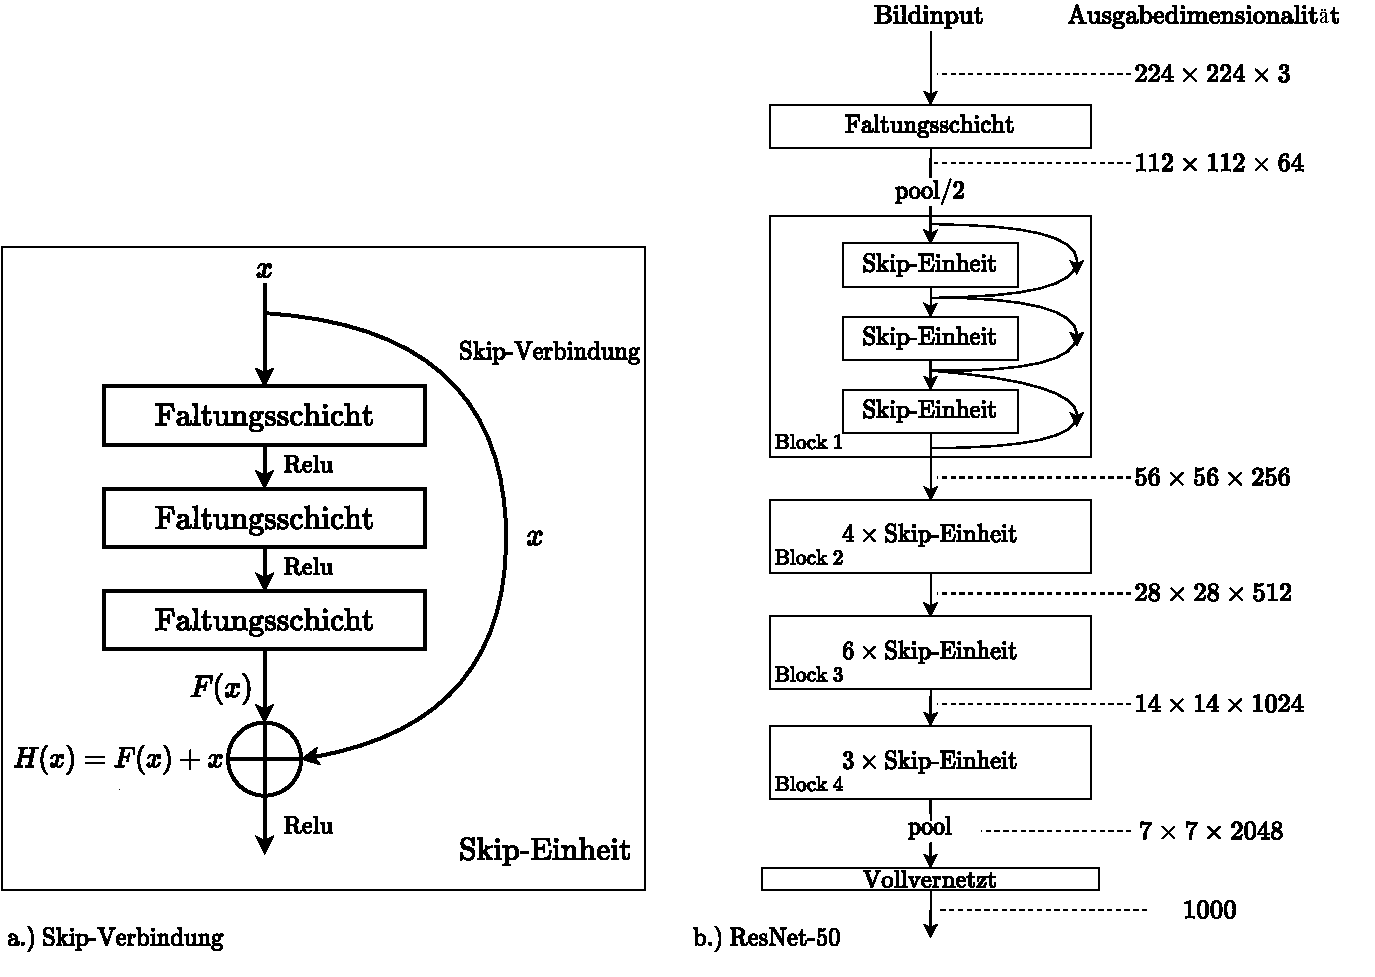
\includegraphics[scale=0.70]{resnet-50.pdf}
\caption{Aufbau der ResNet-Architektur (vgl. Fig.2, Fig.3 aus \cite{resnet})}
\end{figure}

\end{document}